\chapter*{Chapitre 1: Contexte général}       
\addcontentsline{toc}{chapter}{Chapitre 1: Contexte général}  
\stepcounter{chapter} 

% ======= Introduction =======
\section{Introduction}
Ce chapitre présente le contexte général de mon stage, en introduisant l'entreprise d'accueil, son secteur d'activité et l'environnement dans lequel j'ai évolué. Mon stage s'est déroulé à distance, avec des réunions quotidiennes (daily standups) et l'utilisation d'outils de communication et de gestion tels que Git et GitHub, permettant une collaboration efficace malgré la distance.\\[1mm]
L'entreprise \textbf{\textcolor{ftRed}{FeverTokens}}, située en France, est spécialisée dans le développement de solutions Web 3.0 et blockchain. Ce chapitre détaillera sa présentation, son organisation interne, le département auquel j'étais rattaché, ainsi que les objectifs et missions de mon stage.\\[.5cm]


% ======= Présentation =======
\section{Présentation de l'entreprise et du secteur}
    \leftskip.75cm
    \subsection{Présentation de l'entreprise}
    \vskip.5cm
    \begin{figure}[h]
        \centering
        
\includegraphics[width=.6\textwidth]{figures/fevertokens_logo.pdf}
        \caption{Logo de FeverTokens}
        \label{fig:fevertokens_logo}
    \end{figure}
    \vskip.25cm
    \textbf{\textcolor{ftRed}{FeverTokens}} est une entreprise française spécialisée dans la blockchain qui propose des solutions open-source innovantes pour le développement Web3. Elle utilise des technologies avancées de smart contracts et de formal verification afin de garantir des applications sécurisées et performantes. L'entreprise se positionne comme un acteur majeur dans le développement de protocoles blockchain de niveau application, notamment pour la tokenisation d'actifs réels. Son \textit{protocol builder} soutient déjà des projets sophistiqués et hautement scalables, permettant aux développeurs de créer des applications Web3 avancées avec efficacité et sécurité.\\[5mm]
    Au coeur de son activité se trouve le \textit{Package-Oriented Web3 Framework}, un cadre modulaire qui facilite le développement et le déploiement de smart contracts et d'applications décentralisées. Cette architecture permet de combiner flexibilité, modularité et sécurité intégrée, tout en s'inspirant des bonnes pratiques des logiciels Web2 matures.\\[5mm]
    L'environnement de travail chez \textbf{\textcolor{ftRed}{FeverTokens}}.io est à la fois technique et collaboratif. Les équipes partagent un climat de confiance et de soutien mutuel, favorisant l'échange d'idées et la résolution collective des problèmes. Même en travaillant à distance, la cohésion reste forte grâce aux réunions quotidiennes, aux outils de communication sophistiqués, et à une culture d'entraide qui encourage chacun à progresser et à apprendre. Cette atmosphère permet un apprentissage continu et la réalisation de projets complexes dans un cadre motivant et stimulant.
    
    \subsection{Secteur}
    \textbf{\textcolor{ftRed}{FeverTokens}} évolue dans le secteur technologique, en particulier dans le domaine de l'information et de l'Internet. L'entreprise se spécialise dans la blockchain et les technologies Web3, développant des solutions avancées pour la création et la gestion de smart contracts et d'applications décentralisées. Elle offre un environnement de travail collaboratif et stimulant, favorisant l'échange d'idées, l'apprentissage continu et la réalisation de projets complexes dans un cadre motivant.


    \subsection{Spécialités et solutions}
    L'entreprise se distingue par ses spécialités variées dans le domaine de la blockchain et du Web3. Elle travaille sur des projets liés aux NFT, Metaverse, marketplaces, SDK, smart contracts, crypto-monnaies et actifs numériques. \textbf{\textcolor{ftRed}{FeverTokens}} met également l'accent sur l'intelligence artificielle et la tokenisation, offrant des solutions no-code qui permettent aux développeurs et aux entreprises de créer facilement des applications sécurisées, flexibles et rapides. Son approche unique garantit à la fois une scalabilité fonctionnelle et une sécurité de niveau entreprise grâce à la vérification formelle. Pour plus d'informations, le site web officiel de l'entreprise est accessible à l'adresse \textcolor{ftBlue}{\url{https://fevertokens.io}}.\\[.5cm]

\leftskip0cm

% ======= Organisation interne =======
\section{Structure Organisationnelle}
    \leftskip.75cm
    \subsection{Organigramme simplifié}
    \vskip.5cm
     \begin{figure}[h]
        \centering
        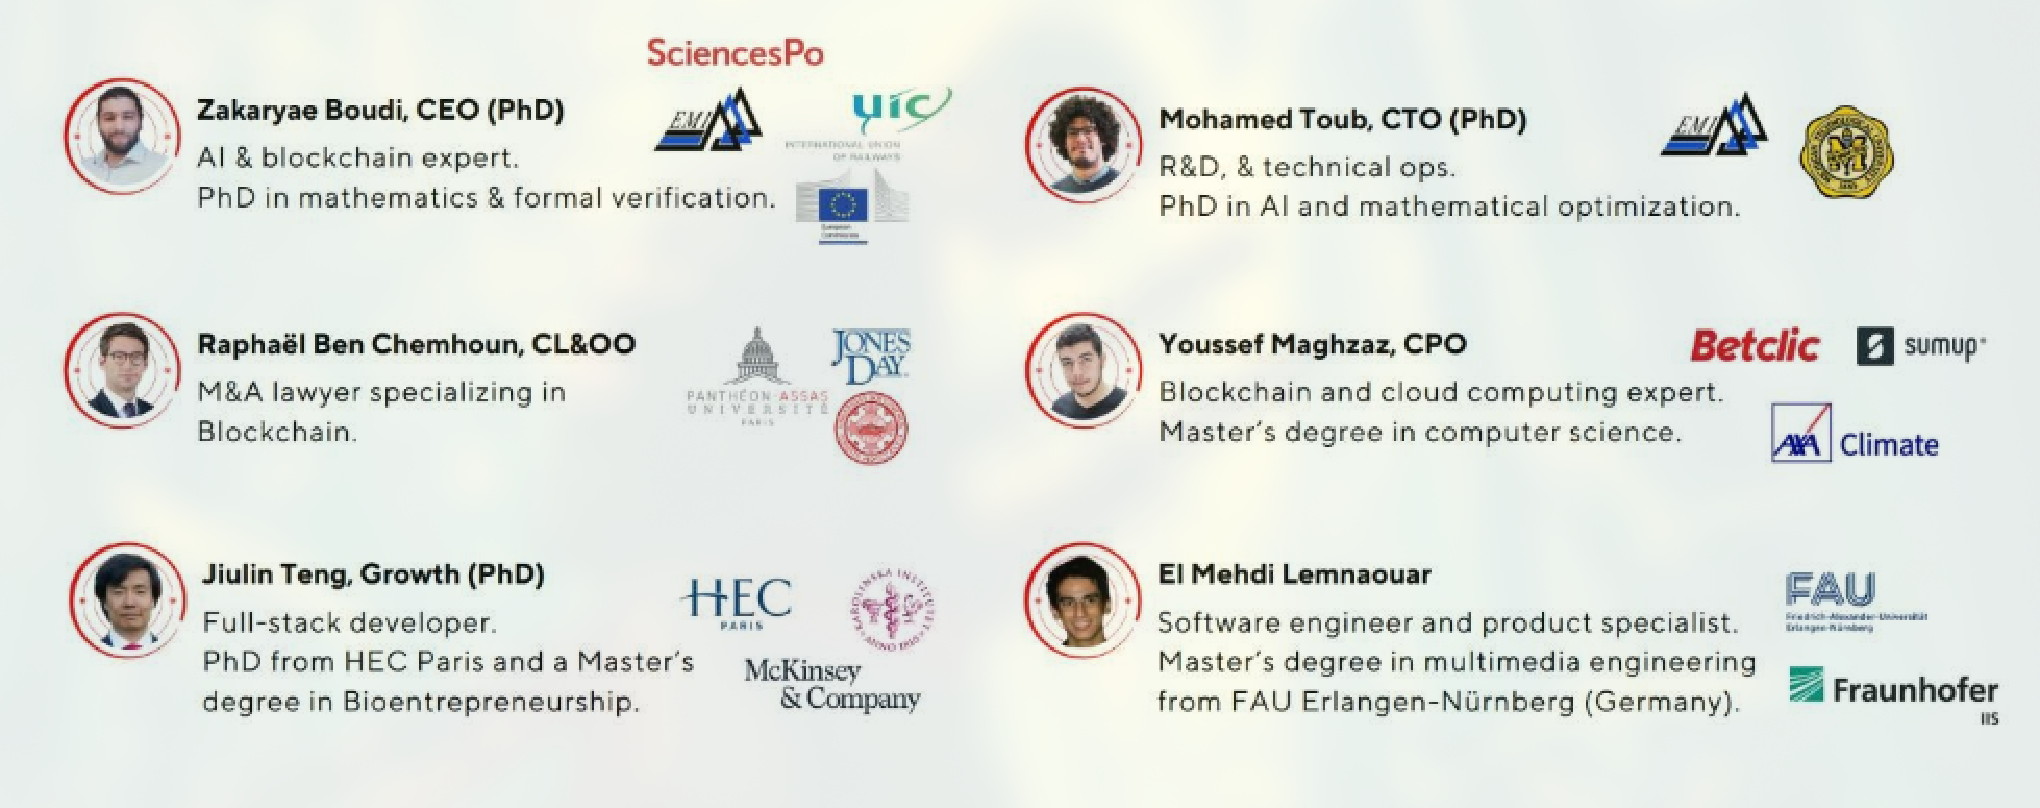
\includegraphics[width=.6\textwidth]{figures/fevertokens_team.pdf}
        \caption{Team de FeverTokens}
        \label{fig:fevertokens_team}
    \end{figure}
    \vskip.25cm
    L'entreprise \textbf{\textcolor{ftRed}{FeverTokens}} est dirigée par son CEO, \textbf{Zakaryae Boudi}, expert en intelligence artificielle et blockchain, titulaire d'un doctorat en mathématiques et en vérification formelle. Sous sa direction, le CTO, \textbf{Dr. Mohamed Toub}, supervise la recherche et les opérations techniques de l'entreprise.\\[2mm]
    L'équipe technique comprend \textbf{Youssef Maghzaz}, expert en blockchain et cloud computing, et \textbf{El Mehdi Lemnaouar}, ingénieur logiciel et spécialiste produit, responsable du suivi des réunions quotidiennes et de la coordination de l'équipe. Mon rôle en tant que stagiaire full-stack se situe au sein de cette équipe technique spécialisée dans le développement d'applications Web3 et cloud.

    \subsection{Mon département/équipe}
    J'ai été intégré au département des \textbf{développeurs full-stack}, qui constitue le coeur du développement logiciel chez \textbf{\textcolor{ftRed}{FeverTokens}}. L'équipe est petite mais hautement spécialisée et collaborative. Ses principales missions incluent le développement d'applications Web3 sécurisées, la mise en oeuvre de smart contracts modulaires, et la maintenance de l'infrastructure cloud associée.\\[2mm]
    Le travail se déroule dans un environnement technique stimulant et collaboratif, où les échanges d'idées sont fréquents et où chacun contribue à la résolution collective des problèmes. Les réunions quotidiennes et les outils de communication sophistiqués permettent à l'équipe de rester synchronisée et efficace, même en télétravail. Mon rôle principal consistait à développer des fonctionnalités full-stack, en respectant les bonnes pratiques de code structuré et propre.\\[.5cm]

\leftskip0cm

% ======= Objectifs et missions =======
\section{Mandat du stage et objectifs}
\vskip1mm
Le mandat de ce stage consistait à m'intégrer au sein de l'équipe de développement full-stack afin de contribuer à l'évolution des projets de l'entreprise et d'acquérir une expérience pratique dans un environnement professionnel.\\[5mm]
Les objectifs principaux étaient :
\begin{itemize}
  \leftskip.75cm
    \item Approfondir mes compétences en développement \textbf{full-stack}, notamment autour de \textbf{Next.js} et des architectures en \textbf{monorepo}.
    \item Participer à la conception et à l'amélioration de modules liés à la \textbf{base de données} et à l'\textbf{interface utilisateur}.
    \item Développer ma capacité à travailler en \textbf{équipe}, en collaborant avec des développeurs experts et d'autres stagiaires.
    \item Découvrir et appliquer de bonnes pratiques de \textbf{structuration du code} et de \textbf{gestion de projet} dans un cadre professionnel.
    \item Assister aux \textbf{présentations techniques} encadrées et profiter de ces expériences pour progresser dans l'art de présenter et partager des idées efficacement.
\end{itemize}
\leftskip0cm
\clearpage

% ======= Conclusion =======
\section{Conclusion}
Ce chapitre a présenté le contexte général de mon stage, en détaillant l'entreprise \textbf{\textcolor{ftRed}{FeverTokens}}, son secteur d'activité, sa structure organisationnelle ainsi que les objectifs et missions qui m'ont été confiés. Il met en lumière l'environnement technique et collaboratif dans lequel j'ai évolué, posant les bases de la compréhension des travaux développés dans les chapitres suivants.
\clearpage